% !TEX program = xelatex
\documentclass[a4paper, notitlepage]{article}
\usepackage{geometry}
\geometry{a4paper,scale=0.6}
\usepackage[]{xeCJK}
\usepackage{cite}
\usepackage{setspace}
\usepackage{indentfirst}
\usepackage{graphicx}
\usepackage{subfigure}
\usepackage{caption}
\usepackage[noend]{algpseudocode}
\usepackage{algorithmicx,algorithm}
\usepackage{booktabs}

\setCJKmainfont{思源宋体 CN}
\renewcommand{\refname}{参考文献}
\renewcommand{\tablename}{表.}
\renewcommand{\figurename}{图.}
\renewcommand{\thetable}{\arabic{table}}
\renewcommand{\thefigure}{\arabic{figure}}
%\newcommand{\upcite}[1]{\textsuperscript{\textsuperscript{\cite{#1}}}}
\newcommand{\upcite}[1]{\cite{#1}}
\newcommand{\tabincell}[2]{\begin{tabular}{@{}#1@{}}#2\end{tabular}}  

\linespread{1.2}
\begin{document}

\setlength{\parindent}{0pt}
\begin{center}
	\LARGE\textbf{生物智能与算法 Report-3}
\end{center}
\vspace{1em}

\begin{center}
	\textbf{赵昱 21821275}
\end{center}

\setlength{\parindent}{2em}

\section{目标检测问题简介}
目标检测问题分为两个阶段,即目标定位(确定目标所在位置,回归问题)
和目标分类(确定候选框内的目标所属类别),常规方法通常采用滑动窗口加人工
特征分类器进行检测。

YOLO系列\cite{1,2,3}是首个使用单个CNN模型同时处理回归和分类两个问题的神经网络模型。

本项目选择YOLO系列作为多类别目标检测(通常叫做通用目标检测)所采用的模型,尝试复现每个版本并进行比较,同时针对
一些特殊应用(如人脸检测等单类别问题),根据自己的需求训练模型。

\subsection{目标检测问题模型和求解思路}
\subsubsection{问题模型}
目标检测问题要求检测到某类物体在图像中是否存在,并且给出其所在位置的包围框(Bounding Box)。
目标检测问题的模型分为两个阶段,即目标定位(确定目标所在位置,回归问题) 和目标分类(确定候选框内的目标所属类别)。
\begin{figure}[H]
    \centering
    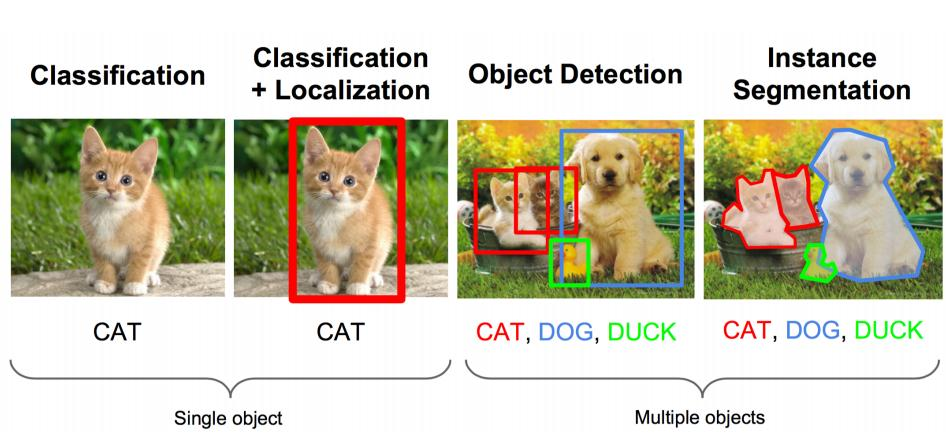
\includegraphics[scale=0.4]{fig_problem_model}
    \caption{目标检测问题模型}
    \label{fig:example}
\end{figure}
常规方法的第一个阶段通常采用滑动窗口的方法来穷举包围框,由于物体的大小不一,滑动窗口的尺寸也会不断变化(在具体实现上,是通过缩放图像,如计算图像金字塔实现的)

在此基础上,使用人工特征分类器进行检测(分类),如使用基于Haar特征的分类器判断是否为人脸,基于HOG特征的分类器判断是否为行人等。

对于常规方法的改进,通常可以从这两个阶段着手。如针对目标定位的改进,有RCNN的Selective Search,Fast RCNN的Region Proposal,或直接将其看成一个回归问题。针对分类器的改进,则通常使用更高层次或更复杂的特征,如使用CNN提取的特征。但是根据包围框候选策略得到的包围框通常不会完全贴合目标的边缘,所以很多方案会进行Bounding Box Regression(位置精修),来得到更加准确的包围框。

\subsubsection{检测结果后处理(Post Processing)}
非极大值抑制(Non-Maximum Suppression,NMS) 滑动窗口经提取特征,经分类器分类识别后,每个窗口都会得到一个分数。但是滑动窗口会导致很多窗口与其他窗口存在包含或者大部分交叉的情况。这时就需要用到NMS来选取那些邻域里分数最高(是目标的概率最大),并且抑制那些分数低的窗口。 NMS在计算机视觉领域有着非常重要的应用,如视频目标跟踪、数据挖掘、3D重建、目标识别以及纹理分析等。 常用的IOU阈值是 0.3 ~ 0.5

\subsection{评估标准}
常见的分类问题,通常使用混淆矩阵来表示分类的结果,即每个类别被分类的结果与真实结果的对比。
对于二分类的混淆矩阵,可以计算召回率(Recall)、精确率(Precision),前者是真实样本被检出的概率,后者则是检出的准确率。
\begin{figure}[H]
    \centering
    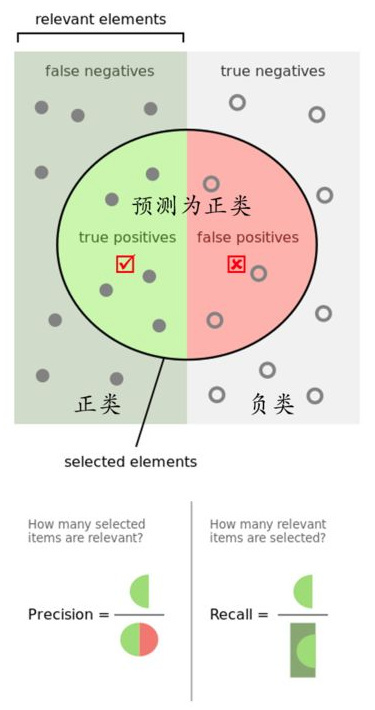
\includegraphics[scale=0.4]{fig_precision_recall}
    \caption{召回率和准确率}
    \label{fig:example}
\end{figure}
在此基础上,还可以计算PR曲线,ROC曲线,F指标等。

以上是针对分类算法的判别标准,评价一个检测算法时,主要看两个指标,即是否正确的预测了框内物体的类别;预测的框和人工标注框的重合程度,故需要以下两个评价标准:
\begin{itemize}
	\item IOU(Intersection Over Union): 用来衡量预测的物体框和真实框的重合程度(通常我们规定IOU > 0.5表示物体被检测出来,否则没有。调整IOU的阈值可以得到PR曲线。)
	\item 平均精度均值(Mean Average Precision,mAP):mAP即是把每个类别的AP都单独拿出来,然后计算所有类别AP的平均值,代表着对检测到的目标平均精度的一个综合度量。(AP的计算方法之一:11点插值法。就是选取0,0.1,0.2…1,这样的11个点,分别对应不同的recall级别,根据不同的级别计算最大Precision(最大是指左侧最大),然后求出它的平均值。)
\end{itemize}

\subsection{目标}
(1):精读论文,理解模型,分析方法的优缺点和创新之处

(2):复现论文

(3):和其他方法进行对比实验

\subsection{论文摘要与翻译}
\subsubsection{[YOLO v1-CVPR2016] You Only Look Once: Unified, Real-Time Object Detection}
\textbf{Abstract:}

We present YOLO, a new approach to object detection.
Prior work on object detection repurposes classifiers to perform
detection. Instead, we frame object detection as a regression
problem to spatially separated bounding boxes and
associated class probabilities. A single neural network predicts
bounding boxes and class probabilities directly from
full images in one evaluation. Since the whole detection
pipeline is a single network, it can be optimized end-to-end
directly on detection performance.

Our unified architecture is extremely fast. Our base
YOLO model processes images in real-time at 45 frames
per second. A smaller version of the network, Fast YOLO,
processes an astounding 155 frames per second while
still achieving double the mAP of other real-time detectors.
Compared to state-of-the-art detection systems, YOLO
makes more localization errors but is less likely to predict
false positives on background. Finally, YOLO learns very
general representations of objects. It outperforms other detection
methods, including DPM and R-CNN, when generalizing
from natural images to other domains like artwork.

\textbf{摘要翻译:}

我们提出YOLO——一种新的目标检测方法。
以前的目标检测工作重新利用分类器来执行检测。
相反,我们将目标检测框架看作回归问题从空间上
分割边界框和相关的类别概率。
单个神经网络在一次评估中直接从完整图像
上预测边界框和类别概率。
由于整个检测流程是单一网络,因此可以直接对检测性能进行端到端的优化。

我们的单一网络架构非常快。
我们的基础YOLO模型以45帧/秒的速度实时处理图像。
网络的一个较小版本,快速YOLO,每秒能处理惊人的155帧,
同时实现其它实时检测器两倍的mAP。
与最先进的检测系统相比,YOLO产生了更多的定位误差,
但不太可能在背景上的预测假阳性。
最后,YOLO学习目标非常通用的表示。
当从自然图像到艺术品等其它领域泛化时,
它都优于其它检测方法,包括DPM和R-CNN。

\subsubsection{[YOLO v2-CVPR2017] YOLO9000: Better, Faster, Stronger}
\textbf{Abstract:}

We introduce YOLO9000, a state-of-the-art, real-time
object detection system that can detect over 9000 object
categories. First we propose various improvements to the
YOLO detection method, both novel and drawn from prior
work. The improved model, YOLOv2, is state-of-the-art on
standard detection tasks like PASCAL VOC and COCO. Us
ing a novel, multi-scale training method the same YOLOv2
model can run at varying sizes, offering an easy tradeoff
between speed and accuracy. At 67 FPS, YOLOv2 gets
76.8 mAP on VOC 2007. At 40 FPS, YOLOv2 gets 78.6
mAP, outperforming state-of-the-art methods like Faster R-
CNN with ResNet and SSD while still running significantly
faster. Finally we propose a method to jointly train on object detection and classification. Using this method we train
YOLO9000 simultaneously on the COCO detection dataset
and the ImageNet classification dataset. Our joint training
allows YOLO9000 to predict detections for object classes
that don’t have labelled detection data. We validate our
approach on the ImageNet detection task. YOLO9000 gets
19.7 mAP on the ImageNet detection validation set despite
only having detection data for 44 of the 200 classes. On
the 156 classes not in COCO, YOLO9000 gets 16.0 mAP.
YOLO9000 predicts detections for more than 9000 different
object categories, all in real-time.

\textbf{摘要翻译:}

我们提出YOLO9000,
这是一种先进的、实时的目标检测系统,
可以检测超过9000个类别。
首先,我们对YOLO做了一些改进,
得到了提升后的模型YOLO v2,
这是一种在如Pascal VOC以及COCO等任务上表现出色,
使用一种新奇的、多尺度的训练方法,
YOLO v2可以适应不同的尺寸,
可以在速度与精度之间提供一个很好的平衡。
在67帧率的时候,YOLO V2 可以获得76.8的mAP在VOC2007上,
40帧率的时候,可以获得78.6的mAP值,
这比Faster R-cnn要好。
最后,我们提出了一种联合训练的方法来进行目标检测和分类。
使用这种方法,我们训练了YOLO 9000,
它可以在ImageNet和COCO上同时进行训练,
我们的这种联合训练方法允许YOLO9000可以进行无标签目标的预测。
我们在ImageNet检测任务中验证了我们的方法,
在44类已有数据集中YOLO9000获得了19.7的mAP值,
在其余的156类没有的样本中,获得了16.0的mAP值。
但是YOLO9000可不是只能预测200类数据,
它可以同时检测出9000种目标,并且仍然可以实时的进行。

\subsubsection{[YOLO v3-(arxiv)2018] YOLOv3: An Incremental Improvement}
\textbf{Abstract:}

We present some updates to YOLO! We made a bunch
of little design changes to make it better. We also trained
this new network that’s pretty swell. It’s a little bigger than
last time but more accurate. It’s still fast though, don’t
worry. At 320 x 320 YOLOv3 runs in 22 ms at 28.2 mAP,
as accurate as SSD but three times faster. When we look
at the old .5 IOU mAP detection metric YOLOv3 is quite
good. It achieves 57:9 AP50 in 51 ms on a Titan X, compared
to 57:5 AP50 in 198 ms by RetinaNet, similar performance
but 3.8x faster. As always, all the code is online at
https://pjreddie.com/yolo/.

\textbf{摘要翻译:}

本文为YOLO提供了一系列更新!
它包含一堆小设计,可以使系统的性能得到更新;
也包含一个新训练的、非常棒的神经网络,
虽然比上一版更大一些,但精度也提高了。
不用担心,虽然体量大了点,它的速度还是有保障的。
在输入320×320的图片后,YOLOv3能在22毫秒内完成处理,
并取得28.2mAP的成绩。它的精度和SSD相当,但速度要快上3倍。
和旧版数据相比,v3版进步明显。
在Titan X环境下,YOLOv3的检测精度为57.9AP,用时51ms;
而RetinaNet的精度只有57.5AP,但却需要198ms,
相当于YOLOv3的3.8倍。

\section{精读论文}
\subsection{[YOLO v1-CVPR2016] You Only Look Once: Unified, Real-Time Object Detection}
\textbf{方法:}
单阶段(one-stage)目标检测。YOLO将目标检测重新定义为单个回归问题,从图像像素直接到边界框坐标和类概率。
\begin{figure}[H]
    \centering
    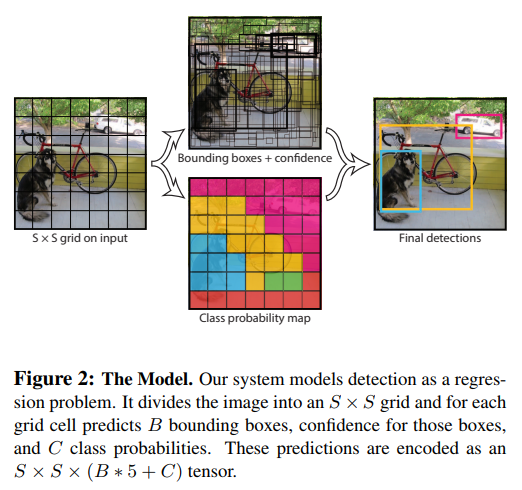
\includegraphics[scale=0.4]{fig_structure_yolov1}
    \caption{方法}
    \label{fig:example}
\end{figure}
\textbf{特色:}
\begin{itemize}
	\item 在预训练的时候用的是224x224的输入,
	一般预训练的分类模型都是在ImageNet数据集上进行的,
	然后在检测的时候采用448x448的输入
	\item 在图像上运行单个卷积网络
	\item 根据模型的置信度对得到的检测进行阈值化。
	(输出为BB+类概率) 
\end{itemize}
\begin{figure}[H]
    \centering
    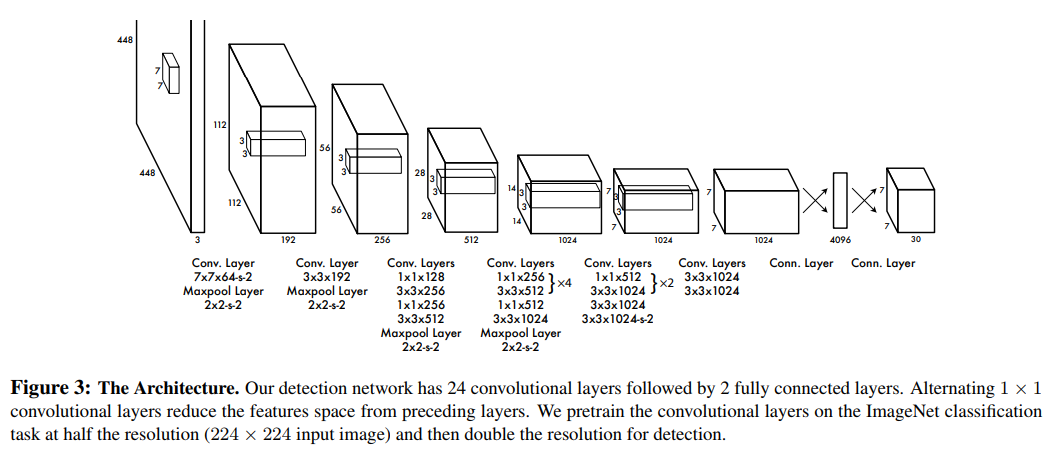
\includegraphics[scale=0.4]{fig_model_yolov1}
    \caption{特色}
    \label{fig:example}
\end{figure}
\textbf{结果:}
\begin{figure}[H]
    \centering
    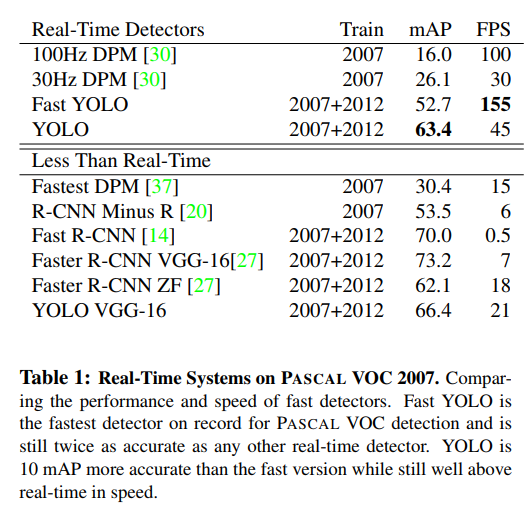
\includegraphics[scale=0.4]{fig_result_yolov1}
    \caption{结果}
    \label{fig:example}
\end{figure}

\subsection{[YOLO v2-CVPR2017] YOLO9000: Better, Faster, Stronger}

\textbf{特色:}
\begin{itemize}
	\item Batch Normalization
	\item High Resolution Classifier:预训练分成两步:先用224*224的输入从头开始训练网络,大概160个epoch,然后再将输入调整到448*448,再训练10个epoch。最后再在检测的数据集上fine-tuning,也就是检测的时候用448*448的图像作为输入就可以顺利过渡了。
	\item Convolutional With Anchor Boxes 
	\item Dimension Clusters:Faster R-CNN中anchor box的大小和比例是按经验设定的,然后网络会在训练过程中调整anchor box的尺寸。
	如果一开始就能选择到合适尺寸的anchor box,那肯定可以帮助网络更好地预测。所以作者采用k-means的方式对训练集的bounding boxes做聚类,试图找到合适的anchor box。
\end{itemize}
\begin{figure}[H]
    \centering
    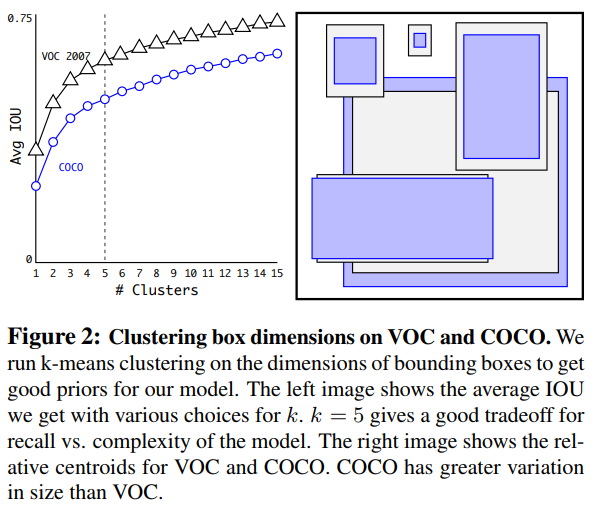
\includegraphics[scale=0.4]{fig_anchor_yolov2}
    \caption{anchor}
    \label{fig:example}
\end{figure}
\begin{figure}[H]
    \centering
    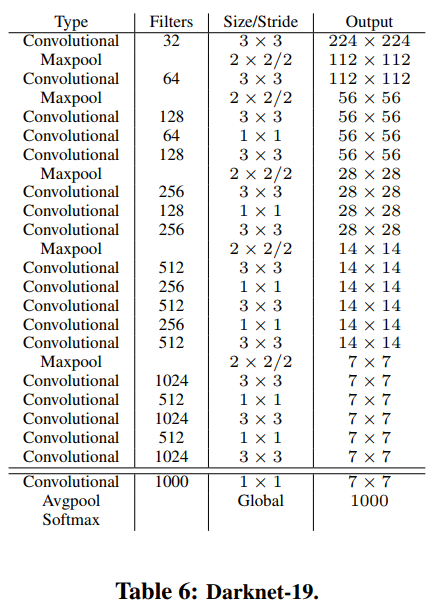
\includegraphics[scale=0.4]{fig_backbone_yolov2}
    \caption{backbone}
    \label{fig:example}
\end{figure}
\textbf{结果:}
\begin{figure}[H]
    \centering
    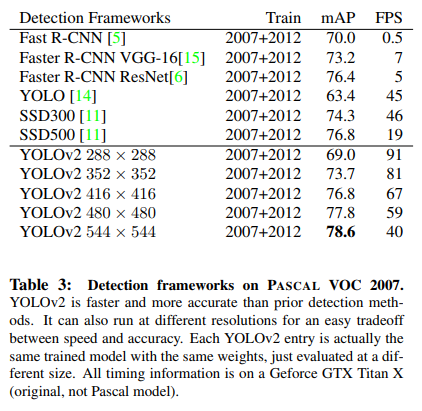
\includegraphics[scale=0.4]{fig_result_yolov2}
    \caption{结果}
    \label{fig:example}
\end{figure}


\subsection{[YOLO v3-(arxiv)2018] YOLOv3: An Incremental Improvement}

\textbf{特色:}
\begin{itemize}
	\item 借鉴了残差网络结构,形成更深的网络层次。
	\item 9种尺度的先验框,mAP以及对小物体的检测效果有一定的提升。
\end{itemize}
\begin{figure}[H]
    \centering
    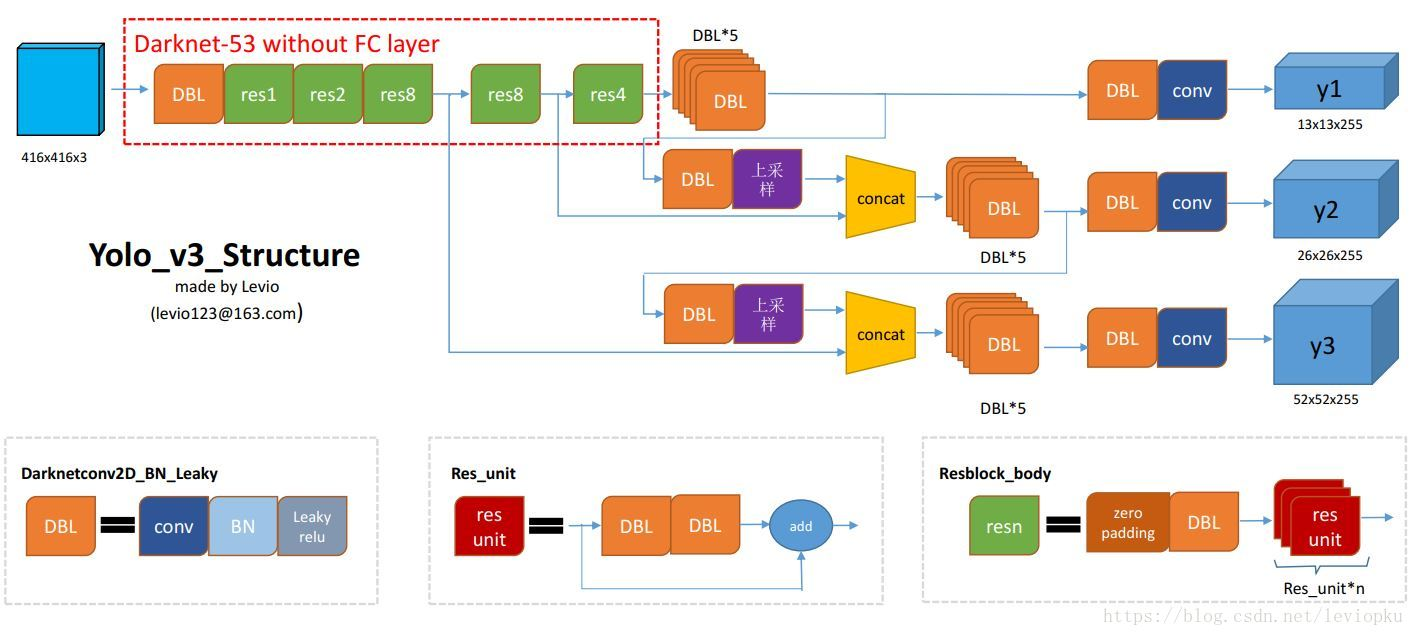
\includegraphics[scale=0.4]{fig_model_yolov3}
    \caption{model}
    \label{fig:example}
\end{figure}
\begin{figure}[H]
    \centering
    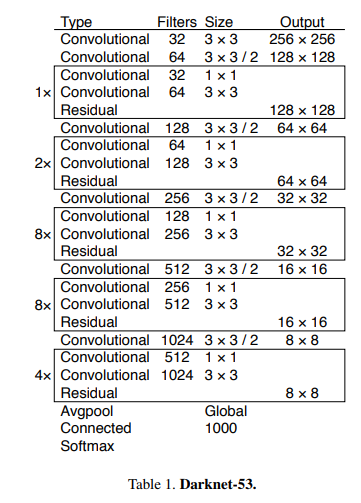
\includegraphics[scale=0.4]{fig_backbone_yolov3}
    \caption{backbone}
    \label{fig:example}
\end{figure}
\textbf{结果:}
\begin{figure}[H]
    \centering
    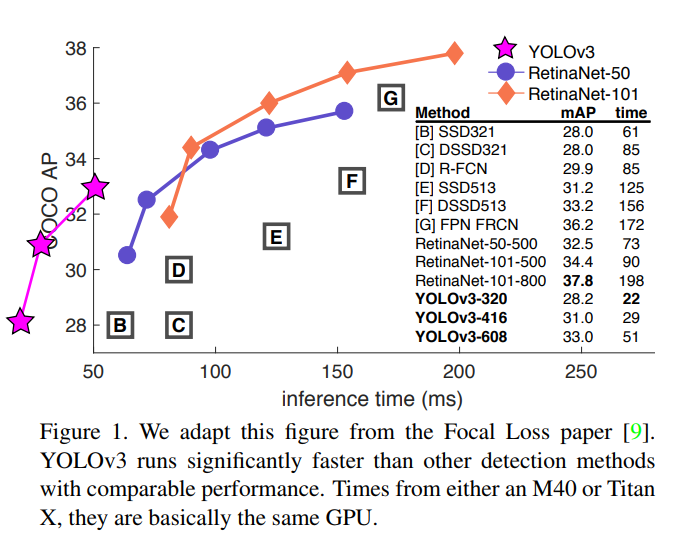
\includegraphics[scale=0.4]{fig_result_yolov3}
    \caption{结果}
    \label{fig:example}
\end{figure}

\section{论文创新点分析与复现}

\subsection{改进目标}
如之前所描述的,目标检测为题分为两个阶段,
即目标定位(确定目标所在位置,回归问题)
和目标分类(确定候选框内的目标所属类别),
因此改进通常针对这两个阶段进行:

\begin{table}[H]
    \caption{目标检测问题改进}
    \centering
    \begin{tabular}{ccc}
        \toprule
        {类别} & {改进点} & {举例}\\
        \midrule
        目标定位 & \tabincell{c}{高效定位\\
                        边框回归\\减少重复}
                         & 
                         \tabincell{c}{
                             Sliding Window\\
                            Selective Search\\
                            Region Proposal\\
                        BB Regression\\
                        NMS
                        }\\
        目标分类  & \tabincell{c}{
            高层特征\\
            多尺度} & \tabincell{c}{
                                Haar\\
                                SIFT\\
                            CNN(VGG、ResNet)\\
                            Image Pyramid
                            } \\
        \bottomrule
    \end{tabular}
\end{table}

\subsection{单阶段网络的定位改进}
YOLO将目标检测重新定义为单个回归问题(one-stage object detection),从图像像素直接到边界框坐标和类概率。
这种方法最大的特点是不需要一一确定包围框(region proposal)的
位置,因此效率较高,但主要有两个缺点:

(1)定位不准确

(2)和基于region proposal的方法相比召回率较低。

\subsubsection{定位改进——Anchor}
YOLOv1是利用全连接层直接预测bounding box的坐标。

YOLOv2则借鉴了Faster R-CNN的思想,引入anchor。

YOLOv2做了以下改变:

(1)删掉全连接层和最后一个pooling层,使得最后的卷积层可以有更高分辨率的特征;

(2)缩减网络,用416*416大小的输入代替原来448*448。这样做是希望希望得到的特征图都有奇数大小的宽和高,奇数大小的宽和高会使得每个特征图在划分cell的时候就只有一个中心cell。因为大的目标一般会占据图像的中心,所以希望用一个中心cell去预测,而不是4个中心cell。网络最终将416*416的输入下采样32倍变为13*13大小的feature map输出,查看.cfg文件可以看到有8个pooling层。

YOLOv1中将输入图像分成7*7的网格,每个网格预测2个bounding box,一共只有7*7*2=98个box。

YOLOv2中引入anchor boxes,输出feature map大小为13*13,每个cell有5个anchor box预测得到5个bounding box,一共有13*13*5=845个box。增加box数量是为了提高目标的定位准确率。

Faster R-CNN中anchor box的大小和比例是按经验设定的,然后网络会在训练过程中调整anchor box的尺寸。
如果一开始就能选择到合适尺寸的anchor box,那肯定可以帮助网络更好地预测。所以作者采用k-means的方式对训练集的bounding boxes做聚类,试图找到合适的anchor box。

作者发现采用标准的k-means(即用欧式距离来衡量差异),在box的尺寸比较大的时候其误差也更大,而我们希望的是误差和box的尺寸没有太大关系。所以通过IOU定义了距离函数,使得误差和box的大小无关:
设置先验框的主要目的是为了使得预测框与ground truth的IOU更好,所以聚类分析师使用box与聚类中的box之间的IOU值作为距离指标。
在VOC和COCO数据集上的聚类分析结果,随着聚类中心数目的增加,平均IOU值(各个边界框与聚类中心的IOU的平均值)是增加的,但是综合考虑模型复杂度和召回率,作者最终选取5个聚类中心作为先验框。

实验对比:

(1)采用聚类分析得到的先验框比手动设置的先验框平均IOU值更高,因此模型更容易训练学习。

(2)仅选取5种box就能达到Faster RCNN的9种box的效果。


\subsubsection{分类改进——CNN特征}
YOLOv2的总体结构,只有卷积层、降采样层(Maxpooling、Averagepooling)以及一个
shortcut层(细粒度特征):后端网络结构如下图所示:

\begin{figure}[H]
    \centering
    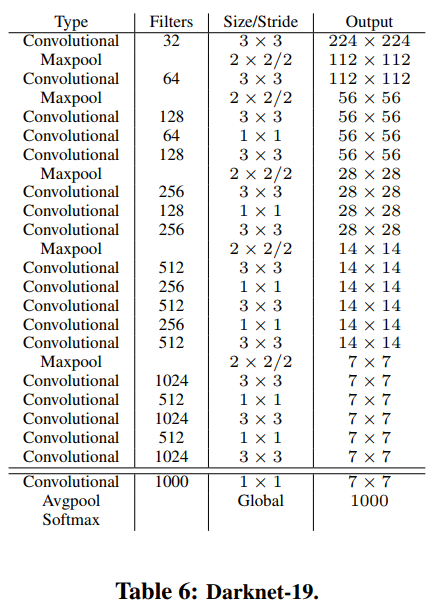
\includegraphics[scale=0.8]{fig_backbone_yolov2}
    \caption{backbone}
    \label{fig:example}
\end{figure}

\subsubsection{分类改进——多尺度训练}
现在基本跑个分类或目标检测模型都不会从随机初始化所有参数开始,所以一般都是用预训练的网络来fine-tuning自己的网络,而且预训练的网络基本上都是在ImageNet数据集上跑的,一方面数据量大,另一方面训练时间久,而且也比较容易得到。

YOLOv1在预训练的时候用的是224*224的输入,一般预训练的分类模型都是在ImageNet数据集上进行的,然后在检测的时候采用448*448的输入。这会导致从分类模型切换到检测模型的时候,模型还要适应图像分辨率的改变。

YOLOv2中将预训练分成两步:先用224*224的输入从头开始训练网络,大概160个epoch,然后再将输入调整到448*448,再训练10个epoch。**注意这两步都是在ImageNet数据集上操作。**最后再在检测的数据集上fine-tuning,也就是检测的时候用448*448的图像作为输入就可以顺利过渡了。

YOLOv2中只有卷积层和池化层,因此不需要固定的输入图片的大小。

为了让模型更有鲁棒性,作者引入了多尺度训练。就是在训练过程中,每迭代一定的次数,改变模型的输入图片大小。

网络输入是416*416,经过5次max pooling之后会输出13*13的feature map,也就是下采样32倍,因此作者采用32的倍数作为输入的size,具体采用320、352、384、416、448、480、512、544、576、608共10种size。

输入图片大小为320*320时,特征图大小为10*10,输入图片大小为608*608时,特征图大小为19*19。
每次改变输入图片大小还需要对最后检测层进行处理,然后开始训练。

这种网络训练方式使得相同网络可以对不同分辨率的图像做检测。

在输入size较大时,训练速度较慢,在输入size较小时,训练速度较快,而multi-scale training又可以提高准确率,因此算是准确率和速度都取得一个不错的平衡。

\subsubsection{综合改进——细粒度特征}

这里添加了一个直通层(passthrough layer),即就是源码中的reorg layer,将前面一层的26*26的特征图和本层13*13的特征图进行连接,与ResNet网络的shortcut类似,以前面更高分辨率的特征图为输入,然后将其连接到后面的低分辨率特征图上。
在13*13的特征图上做预测,虽然对于大目标已经足够了,但对小目标不一定足够好,这里合并前面大一点的特征图可以有效的检测小目标。
具体操作:对于26*26*512的特征图,经passthrough层处理之后就变成了13*13*2048的新特征图(特征图大小变为1/4,而通道数变为以前的4倍),然后与后面的13*13*1024特征图连接在一起形成13*13*3072的特征图,最后在该特征图上卷积做预测。

\subsubsection{综合改进——BN}
BN(Batch Normalization)
层简单讲就是对网络的每一层的输入都做了归一化,
这样网络就不需要每层都去学数据的分布,
收敛会快点。
作者在YOLOv2种为每个卷积层都添加了BN层,
由于BN可以规范模型,
所以加入BN后就把dropout去掉了,
实验证明添加了BN层可以提高2\(\%\)的mAP。

\subsection{论文复现}

\subsubsection{目标}
YOLO是一个多类别的目标检测框架,在复现时,我们
使用它来训练一个效果较好的人脸检测器(单类别)。

\subsubsection{网络结构}
网络的总体结构和之前看到的一致,在每个卷积层后有一个BN层,并且
使用leaky Relu作为激活函数。可以看到网络一共进行了5次降采样,每次的大小为
2x2,因此输入图片的大小必须为32的倍数。

\begin{figure}[H]
    \centering
    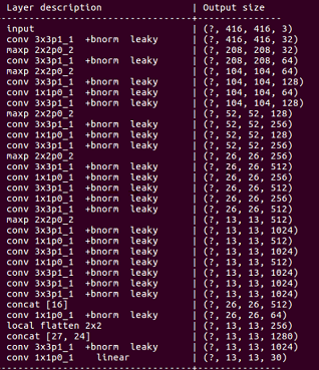
\includegraphics[scale=0.8]{fig_train_network}
    \caption{网络总体结构}
    \label{fig:example}
\end{figure}

\subsubsection{数据集}
数据集为来自直播平台(喵播)的一些实时数据截图,一共
591581张图,使用Face++在线API进行标记,如
下图所示(检测出的人脸区域上至眉心、下至下巴):

\begin{figure}[H]
    \centering
    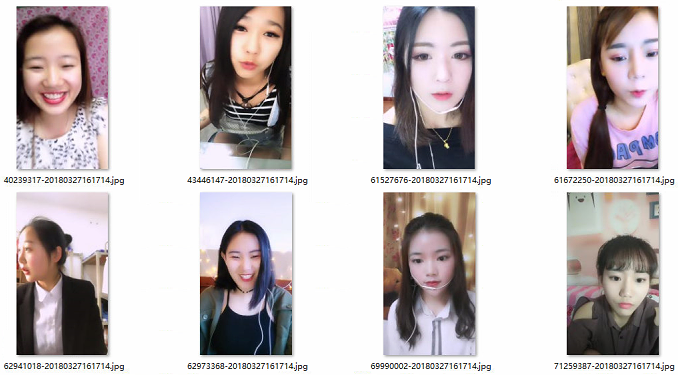
\includegraphics[scale=0.5]{fig_train_dataset}
    \caption{数据集}
    \label{fig:example}
\end{figure}

数据集的标记,即在对应的图片中标记出Bounding Box,一个框使用四个分量表示,如下图所示:
\begin{figure}[H]
    \centering
    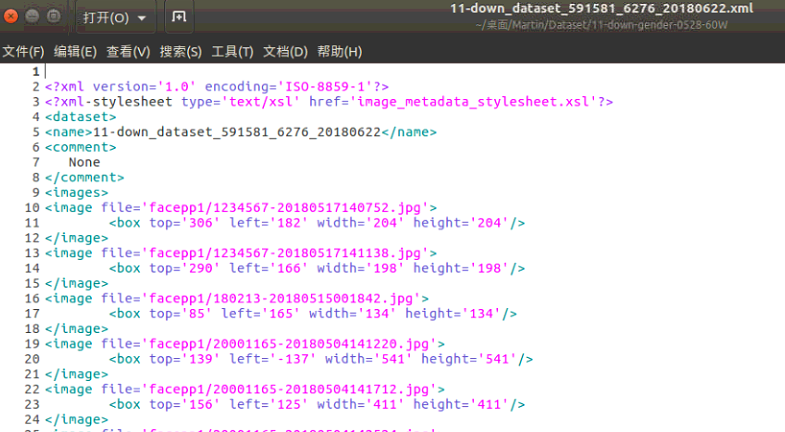
\includegraphics[scale=0.5]{fig_train_label}
    \caption{数据集标记}
    \label{fig:example}
\end{figure}

在数据集中,存在遮挡、低头等较难检测的场景,针对这些数据,
使用手工标注的方式,如下图所示:

\begin{figure}[H]
    \centering
    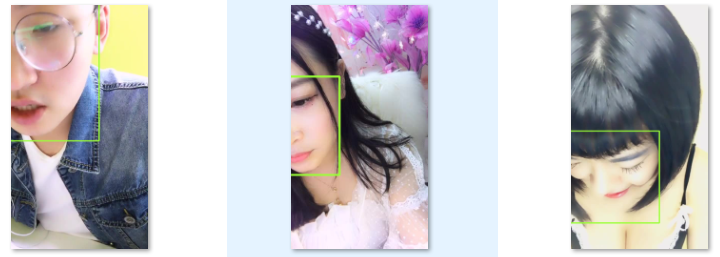
\includegraphics[scale=0.5]{fig_train_hardsample}
    \caption{较困难的样本}
    \label{fig:example}
\end{figure}

\subsubsection{结果}
测试的数据集为来自直播平台(喵播)的一些实时数据截图,一共
120044张图,使用Face++在线API进行标记,有人脸的图片为102680张,算法的表现如下图所示:
\begin{figure}[H]
    \centering
    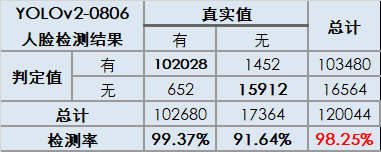
\includegraphics[scale=0.7]{fig_train_result}
    \caption{训练结果}
    \label{fig:example}
\end{figure}

此外,和一些主流的SDK和方案进行了比较,如下图所示:

\begin{figure}[H]
    \centering
    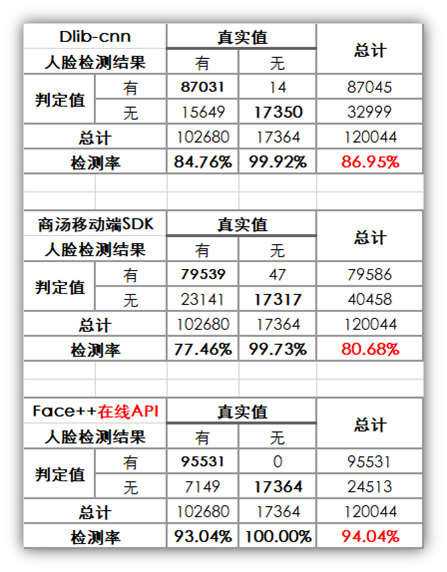
\includegraphics[scale=0.7]{fig_train_compare}
    \caption{与一些方案的比较}
    \label{fig:example}
\end{figure}

\section{方法创新总结与对比试验}
TODO

\begin{thebibliography}{X}
\bibitem{1}
Redmon J, Divvala S, Girshick R, et al. You only look once: Unified, real-time object detection[C]//Proceedings of the IEEE conference on computer vision and pattern recognition. 2016: 779-788.
\bibitem{2}
Redmon J, Farhadi A. YOLO9000: better, faster, stronger[C]//Proceedings of the IEEE conference on computer vision and pattern recognition. 2017: 7263-7271. 
\bibitem{3} 
Redmon J, Farhadi A. Yolov3: An incremental improvement[J]. arXiv preprint arXiv:1804.02767, 2018.
\end{thebibliography}

%\section*{附录 A (若没有附录则删除此章节)}
\clearpage
\bibliography{ref}
\bibliographystyle{unsrt}
\end{document}